\section{Theory}
\label{sec:theory}

The statements below say what the wrapper can and cannot be expected to do, so that the experiments test them and do not merely report outcomes. Each is marked by its status: a statement with a proof is derived; a statement that needs a modelling assumption says which; the last one is a conjecture with its evidence. The proofs are short because the object is a one-dimensional recursion.

\subsection{Coverage with a band: a deterministic identity}
\label{sec:theory-identity}

\begin{proposition}[Coverage identity and bound]
\label{prop:identity}
Run \cref{eq:update} for $n$ days with any model and any sequence of losses, with the band $[\ell, u]$, and let $N_{\mathrm{clip}}$ be the number of days on which the band removed a positive amount, $c_t \ne 0$. Then
\begin{equation}
\frac{1}{n}\sum_{t=t_0}^{t_0+n-1} e_t - \alpha = \frac{a_{t_0} - a_{t_0+n} - C_n}{\gamma\, n}, \qquad C_n = \sum_{t=t_0}^{t_0+n-1} c_t,
\label{eq:identity}
\end{equation}
and consequently
\begin{equation}
\Bigl|\frac{1}{n}\sum_{t} e_t - \alpha\Bigr| \le \frac{u - \ell}{\gamma\, n} + \frac{N_{\mathrm{clip}}}{n}\,\max\{\alpha, 1-\alpha\}.
\label{eq:bound}
\end{equation}
Without clipping ($N_{\mathrm{clip}} = 0$) the bound is $(u-\ell)/(\gamma n)$; the same computation for the unclipped recursion, whose level stays in $[-\gamma, 1+\gamma]$, gives the bound $(\max\{a_1, 1-a_1\} + \gamma)/(\gamma n)$ of \citet{gibbs2021}.
\end{proposition}
\begin{proof}
\Cref{eq:telescoped} is the sum of $a_{t+1} - a_t = \gamma(\alpha - e_t) - c_t$ over the stretch. Solving it for $\sum (\alpha - e_t)$ gives \cref{eq:identity}. Both $a_{t_0}$ and $a_{t_0+n}$ lie in $[\ell, u]$, so $|a_{t_0} - a_{t_0+n}| \le u - \ell$. On a clipped day the raw step $\gamma(\alpha - e_t)$ is $\gamma\alpha$ or $-\gamma(1-\alpha)$, so $|c_t| \le \gamma\max\{\alpha, 1-\alpha\}$ and $|C_n| \le N_{\mathrm{clip}}\,\gamma\max\{\alpha, 1-\alpha\}$. Dividing by $\gamma n$ gives \cref{eq:bound}.
\end{proof}

Two readings follow. The identity is exact, so it can be verified on every run, and it was: on the \thA{} working-level paths of the three models in the stress windows the residual of \cref{eq:identity} is at most $\thAResidual$, and the left side of \cref{eq:bound} is below the right side in \thAHold{} of \thA{} (the check is in \cref{sec:reproducibility}). Second, the bound is informative only for long runs. With the defaults, $(u-\ell)/\gamma = 49.8$, so the first term alone is 0.099 for the 504 days of the longest stress window, ten times the target of 0.01; to bound the error by half of a target of 0.01 the run would need about 10,000 days. For the 18 paths of the experiments the bound of \cref{eq:bound} averages \thAMeanSimple{} percentage points, against targets of 1 and 2.5 points. The coverage improvements reported below are therefore empirical: the proposition shows what is not ruled out, and the experiments show what happened. Where the band was active the proposition names the mechanism by which the guarantee degrades, which is the cut term of \cref{eq:identity}: a lower edge that binds adds a positive amount to the hit frequency, because a cut at the lower edge has $c_t < 0$ and $C_n < 0$.

\subsection{Coverage carries no information on independence}
\label{sec:theory-independence}

\begin{proposition}[A frequency guarantee is compatible with maximal clustering]
\label{prop:independence}
Let $m \ge 2$ be an integer and $\alpha$ a target for which $q = m(1-\alpha)/\alpha$ is an integer. Let the hits be periodic with period $m + q$: $m$ consecutive hits followed by $q$ quiet days. Then (i) the hit frequency is exactly $\alpha$; (ii) if $\gamma m (1-\alpha) < \alpha - \ell$, the sequence is produced by the wrapper of \cref{eq:update} without any clipping, for a model and losses that realise it; (iii) the independence statistic of \citet{christoffersen1998} grows linearly with the length of the sequence, so its p-value tends to zero, while the Kupiec p-value equals one.
\end{proposition}
\begin{proof}
(i) The frequency is $m/(m+q) = m/(m/\alpha) = \alpha$. (ii) For any level in $(0,1)$ the model's VaR is finite by assumption, so the losses can be chosen above it on the $m$ hit days and below it on the quiet days; the hits are then the given ones whatever the model. By \cref{eq:cluster-drop} the level falls by $m\gamma(1-\alpha)$ during a cluster and rises by $q\gamma\alpha = m\gamma(1-\alpha)$ during the quiet days, so the level is periodic with minimum $\alpha - m\gamma(1-\alpha)$, which is above $\ell$ under the stated condition. (iii) Per period the transitions between consecutive days are $n_{00} = q - 1$, $n_{01} = 1$, $n_{10} = 1$, $n_{11} = m - 1$, with sample transition probabilities $\hat\pi_{01} = 1/q$ and $\hat\pi_{11} = (m-1)/m$. The independence likelihood ratio of \citet{christoffersen1998} is
\begin{equation}
\mathrm{LR}_{\mathrm{ind}} = 2\Bigl[\sum_{ij} n_{ij}\ln\hat\pi_{ij} - (n_{00}+n_{10})\ln(1-\hat\pi) - (n_{01}+n_{11})\ln\hat\pi\Bigr], \qquad \hat\pi = \alpha,
\label{eq:lr-ind}
\end{equation}
with $\hat\pi_{i0} = 1 - \hat\pi_{i1}$, and it equals the number of periods times a constant $\kappa(m,\alpha)$ plus a bounded term. The constant is the Kullback--Leibler divergence, times two, of the two-state chain with the empirical transitions from the chain with independent hits at rate $\alpha$, which is positive because $\hat\pi_{11} = (m-1)/m \ge \tfrac12 > \hat\pi_{01}$ for $m \ge 2$ and $q \ge 2$. A positive linear growth of a statistic with a $\chi^2_1$ null gives a p-value that tends to zero. The Kupiec statistic compares the frequency $\alpha$ with the target $\alpha$ and is zero.
\end{proof}

\Cref{tab:cluster} verifies the construction with the engine's own tests on four cases: the Kupiec p-value is 1.000 in all four, the independence p-value is below $10^{-70}$, and the level stays inside the band. The proposition is the reason why the independence test stays among the instruments: a wrapper that satisfies \cref{prop:identity} may deliver exactly the target frequency and still fail the conditional coverage test. It is also a statement about the conditions: for the defaults ($\gamma = 0.005$, $\alpha = 0.01$, $\ell = 0.001$) a cluster of two hits lowers the level by $2\gamma(1-\alpha) = 0.0099$, which exceeds $\alpha - \ell = 0.009$, so the condition of (ii) fails for every $m \ge 2$ and the band clips the level; the cases of \cref{tab:cluster} therefore use the smaller steps $\gamma = 0.001$ at the 1\% level and $\gamma = 0.002$ at the 2.5\% level, for which the condition holds, and the guarantee of the default step is exchanged for the clipping term of \cref{prop:identity}.

\begin{table}[htbp]
\centering
\small
\caption{A hit sequence of clusters of $m$ consecutive hits separated by $q = m(1-\alpha)/\alpha$ quiet days has frequency exactly $\alpha$: the engine's Kupiec test accepts it, its independence test rejects it with a p-value that rounds to zero, and the recursion stays inside the band throughout.}
\label{tab:cluster}
\begin{adjustbox}{max width=\textwidth}
\begin{tabular}{rrrrrrrlr}
\toprule
Level (\%) & Cluster $m$ & Quiet days $q$ & Step $\gamma$ & Days & Hit frequency (\%) & Kupiec $p$ & Independence $p$ & Level range (\%) \\
\midrule
1 & 2 & 198 & 0.001 & 12,000 & 1.00 & 1.000 & 2.2e-94 & 0.802 to 1.000 \\
1 & 3 & 297 & 0.001 & 18,000 & 1.00 & 1.000 & 1.9e-216 & 0.703 to 1.000 \\
2.5 & 2 & 78 & 0.002 & 4,800 & 2.50 & 1.000 & 1.6e-70 & 2.110 to 2.500 \\
2.5 & 4 & 156 & 0.002 & 9,600 & 2.50 & 1.000 & 3.3e-274 & 1.720 to 2.500 \\
\bottomrule
\end{tabular}
\end{adjustbox}
\end{table}


\subsection{Fixed point, repairable scale error and spread of the level}
\label{sec:theory-fixed-point}

Let the standardised loss $Z_t$ have survival function $S$, density $f$ and inverse survival function $\nu(a) = S^{-1}(a)$, with $\nu$ decreasing. Consider a model whose VaR is $V(a) = \sigma\nu(a)$, facing losses $L_t = c\sigma Z_t$ with the $Z_t$ independent and identically distributed, where the scale ratio $c > 0$ is the factor by which the model misjudges the scale of the data. Then the hit probability at level $a$ is
\begin{equation}
G(a) = \Prob\bigl(c\sigma Z > \sigma\nu(a)\bigr) = S\bigl(\nu(a)/c\bigr).
\label{eq:hit-prob}
\end{equation}

\begin{proposition}[Fixed point, band limit and spread]
\label{prop:fixed-point}
Under the model above, with $\ell$ and $u$ not binding: (a) the recursion \cref{eq:update} has the stationary property $\E[G(a_t)] = \alpha$, so the long-run hit frequency equals the target. (b) The rest point of \cref{eq:mean-field} is $a^* = S\bigl(c\,\nu(\alpha)\bigr)$, at which the model's quantile equals the true one, and it is stable. (c) The fixed point lies in the band if and only if $c \le c_{\max} = \nu(\ell)/\nu(\alpha)$. (d) Linearising $G$ around $a^*$, the stationary standard deviation of the level is approximately
\begin{equation}
\mathrm{sd}(a_t) \approx \sqrt{\frac{\gamma\,\alpha(1-\alpha)}{2\,G'(a^*)}}, \qquad G'(a^*) = \frac{f(\nu(\alpha))}{c\,f(c\,\nu(\alpha))}.
\label{eq:spread}
\end{equation}
(e) With the band binding, stationarity of the level gives $\E[G(a_t)] = \alpha - \E[c_t]/\gamma$ with $c_t$ the cut of \cref{eq:telescoped}: a lower edge that binds raises the hit rate above the target by $|\E[c_t]|/\gamma$.
\end{proposition}
\begin{proof}
(a) If the level is stationary, $\E[a_{t+1}] = \E[a_t]$, and taking expectations of \cref{eq:update} without cuts gives $\gamma(\alpha - \E[e_t]) = 0$, with $\E[e_t] = \E[G(a_t)]$ by the tower property. (e) is the same computation with the cut: $\gamma(\alpha - \E[e_t]) - \E[c_t] = 0$. (b) $G(a^*) = \alpha$ means $S(\nu(a^*)/c) = \alpha$, that is $\nu(a^*) = c\,\nu(\alpha)$ and $a^* = S(c\,\nu(\alpha))$. Since $\nu$ is decreasing, $G$ is increasing, $G' = f(\nu(a)/c)/(c\,f(\nu(a))) > 0$, so the right side of \cref{eq:mean-field} is decreasing in $a$ and the rest point is stable. At $a^*$, $\nu(a^*) = c\nu(\alpha)$, which gives the expression of $G'(a^*)$. (c) $a^* \ge \ell$ is $S(c\nu(\alpha)) \ge \ell$, that is $c\,\nu(\alpha) \le \nu(\ell)$. (d) Write $a_t - a^* = x_t$. Then $x_{t+1} = x_t - \gamma\bigl(e_t - G(a_t)\bigr) - \gamma\bigl(G(a_t) - \alpha\bigr) \approx (1 - \gamma G'(a^*))\,x_t - \gamma\xi_t$, where $\xi_t = e_t - G(a_t)$ has mean zero and variance $\alpha(1-\alpha)$ at the rest point. An autoregression of order one with coefficient $\rho = 1 - \gamma G'(a^*)$ and innovation variance $\gamma^2\alpha(1-\alpha)$ has stationary variance $\gamma^2\alpha(1-\alpha)/(1-\rho^2) \approx \gamma\alpha(1-\alpha)/(2G'(a^*))$ for small $\gamma$.
\end{proof}

For the unit-variance Student-$t$ law with five degrees of freedom, $c_{\max}$ is \thCCmaxOne{} at the 1\% level and \thCCmaxTwoHalf{} at the 2.5\% level for the band $[0.001, 0.25]$: a model that underestimates the scale of the data by a factor larger than that cannot be repaired by the wrapper whatever the step. The simulation of \cref{tab:scale-sweep} and \cref{fig:scale-sweep} tests (a) to (e). At $c = 1$ (no scale error) the simulated hit rate is \thCHitUnitOne\% at the 1\% level and \thCHitUnitTwoHalf\% at 2.5\%, and the mean level equals the target. With $c = 1.5$ the fixed point at the 1\% level is $a^* = \thCAstarOne$, inside the band, yet the simulated mean level is \thCMeanOne{} and the hit rate \thCHitOne\%: the spread of the level (simulated \thCSdOne{}, predicted \thCSdPredOne{}) is comparable to the distance of $a^*$ to the lower edge, so the band is active, and the hit rate exceeds the target as part (e) says: the excess of the hit rate over the target is \thCExcessOne{} points at the 1\% level, and the cut term $|\E[c_t]|/\gamma$ computed from the simulated cuts is \thCCutOne{} points (the identity of \cref{eq:identity} holds in every simulated run to \thCIdGap). The condition that (b) describes the behaviour of the unclipped recursion is thus not that $a^*$ is in the band but that $a^* - \ell$ is large against the standard deviation of \cref{eq:spread}. The linearisation overstates the spread by a factor between \thCSdRatioMin{} and \thCSdRatioMax{} of the simulated value (the simulated deviation is smaller), which is the direction expected when the lower edge reflects the level.

\begin{table*}[htbp]
\centering
\small
\caption{A model facing returns $c$ times larger in scale than it assumes (Student-$t$ with five degrees of freedom): the fixed point of the working level, the mean and standard deviation of the level simulated over 50 replications of 5,000 days, the standard deviation predicted by the linearisation, the long-run hit rate with its 95\% interval and the share of updates cut by the band $[0.1\%, 25\%]$.}
\label{tab:scale-sweep}
\begin{adjustbox}{max width=\textwidth}
\begin{tabular}{rrrlrrrlr}
\toprule
Level (\%) & Scale ratio $c$ & Fixed point $a^*$ (\%) & $a^*$ in band & Simulated mean level (\%) & Simulated sd (\%) & Predicted sd (\%) & Hit rate (\%, 95\% CI) & Clipped days (\%) \\
\midrule
1 & 1 & 1.000 & yes & 1.006 & 0.462 & 0.497 & \relax 1.02 $\pm$ 0.01 & 0.1 \\
1 & 1.25 & 0.422 & yes & 0.526 & 0.287 & 0.339 & \relax 1.22 $\pm$ 0.02 & 0.5 \\
1 & 1.5 & 0.197 & yes & 0.355 & 0.196 & 0.239 & \relax 1.61 $\pm$ 0.03 & 1.2 \\
1 & 1.75 & 0.100 & yes & 0.277 & 0.146 & 0.174 & \relax 2.18 $\pm$ 0.04 & 2.0 \\
1 & 2 & 0.055 & no & 0.231 & 0.111 & -- & \relax 2.89 $\pm$ 0.05 & 2.8 \\
1 & 3 & 0.008 & no & 0.160 & 0.056 & -- & \relax 6.71 $\pm$ 0.10 & 6.7 \\
2.5 & 1 & 2.500 & yes & 2.505 & 0.740 & 0.781 & \relax 2.51 $\pm$ 0.02 & 0.0 \\
2.5 & 1.25 & 1.182 & yes & 1.222 & 0.547 & 0.575 & \relax 2.54 $\pm$ 0.01 & 0.1 \\
2.5 & 1.5 & 0.596 & yes & 0.699 & 0.379 & 0.427 & \relax 2.77 $\pm$ 0.02 & 0.7 \\
2.5 & 1.75 & 0.320 & yes & 0.481 & 0.277 & 0.322 & \relax 3.24 $\pm$ 0.03 & 1.7 \\
2.5 & 2 & 0.182 & yes & 0.374 & 0.218 & 0.248 & \relax 3.92 $\pm$ 0.06 & 2.8 \\
2.5 & 3 & 0.029 & no & 0.223 & 0.113 & -- & \relax 7.82 $\pm$ 0.11 & 7.6 \\
\bottomrule
\end{tabular}
\end{adjustbox}
\end{table*}


\begin{figure}[htbp]
\centering
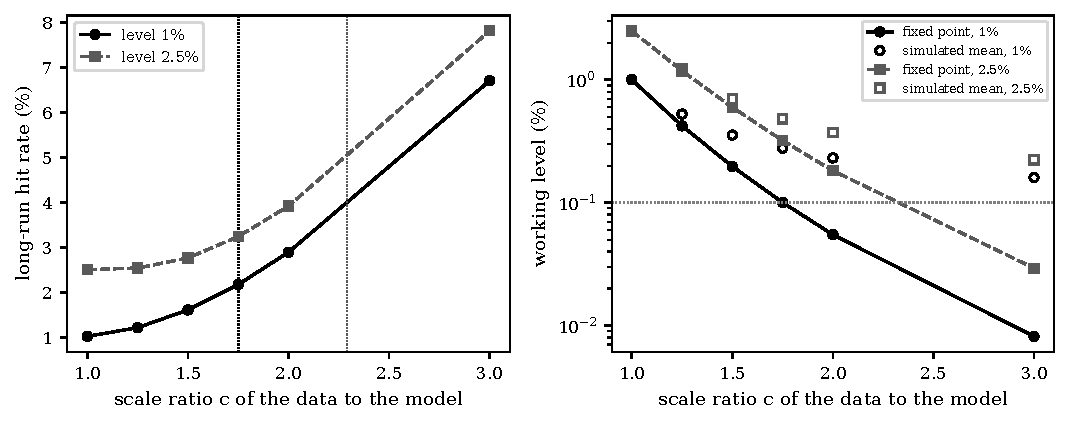
\includegraphics[width=\textwidth]{scale-sweep}
\caption{The wrapper facing a model that misjudges the scale of the data by a ratio $c$ (Student-$t$ with five degrees of freedom, 50 replications of 5,000 days): the long-run hit rate (left) and the fixed point and simulated mean of the working level on a logarithmic axis (right), at the 1\% and 2.5\% levels; the vertical dotted lines mark the largest repairable ratio of each level and the horizontal dotted line the lower edge of the band.}
\label{fig:scale-sweep}
\end{figure}

\subsection{The expected shortfall carried by the working level}
\label{sec:theory-es}

\begin{proposition}[ES at the fixed point of a Pareto tail]
\label{prop:es}
Let the model's tail be exactly a Pareto law of index $\xi < 1$, $V(a) = x_m a^{-\xi}$ and $E(a) = V(a)/(1-\xi)$, facing losses with the same tail shape and a scale $c$ times larger. At the fixed point $a^* = \alpha c^{-1/\xi}$ the wrapped ES equals the true ES at level $\alpha$.
\end{proposition}
\begin{proof}
The true VaR at level $\alpha$ is $c\,x_m\alpha^{-\xi}$ and the fixed point makes $x_m a^{*-\xi}$ equal to it, so $a^* = \alpha c^{-1/\xi}$. Then $E(a^*) = V(a^*)/(1-\xi) = c\,x_m\alpha^{-\xi}/(1-\xi)$, which is the true ES of the scaled law, $c\,E(\alpha)$.
\end{proof}

The Pareto tail is the case in which the ratio $r(a) = E(a)/V(a)$ does not depend on the level, and the proposition is that case: the wrapped ES is exact when the ratio is level-free. When it is not, the ratio of the wrapped ES to the true ES at the fixed point is $r(a^*)/r(\alpha)$. For the Student-$t$ law the ratio $r(a)$ rises with $a$ above its limit $\nu/(\nu-1)$ at $a \to 0$, and since $a^* < \alpha$ the wrapped ES is below the true one. The computation of \cref{sec:reproducibility} (Student-$t$ with 3, 5, 10 and 30 degrees of freedom at $c = 2$ and the 1\% level) gives a ratio of \thDRatioNuThree{}, \thDRatioNuFive{}, \thDRatioNuTen{} and \thDRatioNuThirty{}: an understatement of the ES by 2\% to 8\% that grows with the degrees of freedom, as the tail loses its power-law shape. The monotonicity of $r$ is checked on these four laws and on the two target levels and is not proved for all $\nu$.

\subsection{A conjecture on the score}
\label{sec:theory-conjecture}

\emph{Conjecture.} For a location-scale model with a scale error that the band allows to repair, the expected FZ0 score of the wrapped pair at the fixed point is lower than that of the unwrapped pair, by an amount that grows with $c$ and is largest for the models whose unwrapped ES is furthest from the truth. The evidence is of three kinds. The score of \cref{eq:fz0} is strictly consistent for the pair of the true VaR and ES, so any change that moves the VaR towards the true quantile lowers the expected score as long as the paired ES does not move away from the true ES by more than the VaR gains, and \cref{prop:es} shows that the wrapped ES moves to the true ES for a Pareto tail and stays within a few percent for the Student-$t$ tails. In the generators of known truth the median relative change of the score of the wrapped pair is negative for historical simulation in the three scenarios with a shift and at most \genFzPosMax\% for any model and scenario, which is inside the 5\% tolerance everywhere (\cref{tab:generators}). On the real windows the wrapped pair lowers the mean score in most of the cells, the worst change being \tenWorstFz\% (\cref{fig:fz0-change}). The conjecture is not proved: the condition on the paired ES is the part for which no argument is given, and a counter-example would be a model whose ES at the working level overstates the true ES by more than its VaR gains; the cells of the experiments with a positive change of the score (the filtered models in the generators) are of that kind.

\subsection{Conditions}
\label{sec:theory-conditions}

The statements hold under conditions that the experiments exercise. \Cref{prop:identity} holds for every run and every sequence, with the stated bound; it needs the update to be applied in time order with the hit of the day observed before the next day's level is used. \Cref{prop:independence} concerns the existence of a sequence, and needs $\gamma m(1-\alpha) < \alpha - \ell$ to avoid clipping. \Cref{prop:fixed-point} assumes independent and identically distributed standardised losses and a model that is a pure scale error of the truth; real windows have a changing volatility and a model that may be wrong in shape, so the proposition is a description of a limiting case that the generator experiments and the scale sweep test, not a theorem about the stress windows. \Cref{prop:es} assumes a Pareto tail for both the model and the truth. Two conditions bear on all four statements together. The hit of a day must be known before the level of the next day is used, so a delay in the confirmation of the hit shifts the update and is outside the identity as stated. The model must return a finite VaR and ES at every level of the band: the engine refuses a forecast that is not finite, and the experiments repeat the previous forecast on such a day and count it (\tenFallback{} days in all, in the \tenIndRunsAll{} wrapped runs of the six windows).
